\chapter{Risultati}
\section{Validazione risultati implementazione}
Inizialmente è stata validata l'intera pipeline di Image Captioning implementata con l'obiettivo di verificare il corretto funzionamento e il punto di partenza ottenuto rispetto al modello originale \cite{li2020oscar, zhang2021vinvl}.
Quindi è stato utilizzato lo split \textbf{Karpathy} \cite{karpathy2015deep} sul dataset \acrshort{coco}, questo split prevede una suddivisione in train, validation e test. In questa fase di convalida è stata utilizzata la porzione di test, composta da 5000 immagini con cinque caption ciascuna.
La pipeline è stata testata utilizzando il modello di Object Detection (spiegato nella sezione \ref{object_detection}), per l'estrazione delle feature sulle immagini dello split di test, e \acrshort{oscar}$_+$ fine-tuned su \acrshort{coco} come modello linguistico, sfruttando i pesi resi disponibili dagli autori\footnote{\url{github.com/microsoft/Oscar}} basati sul modello \acrshort{bert} Base.
La decodifica delle caption è stata effettuata utilizzando l'algoritmo Constrained Beam Search (per maggiori dettagli vedere la Sezione \ref{constrained_beam_search}) con dimensione dei beam pari a 5, con lunghezza massima della sequenza pari a 20 e vincolando la decodifica a includere le parole dei tag oggetto q.
Infine, sono state utilizzate le seguenti metriche di valutazione\footnote{Tutte le metriche sono state moltiplicate per cento per consentire una lettura più veloce dei valori. Inoltre, i risultati migliori sono quelli che presentano i valori più alti.}: \textit{\acrshort{bleu}@4} (con @4 si intendono n-grammi con lunghezza massima di 4), \textit{\acrshort{meteor}}, \textit{\acrshort{cider}} e \textit{\acrshort{spice}} (per maggiori dettagli sulle metriche vedere la sezione \ref{metriche}).
%\begin{itemize}
%    \item \textit{BLEU}: è una metrica di precisione modificata con una penalità sulla brevità delle frasi, calcolata come media geometrica ponderata su n-grammi di lunghezza diversa (con BLEU@4 si intendono n-grammi con lunghezza massima di 4);
%    \item \textit{METEOR}: abbina gli unigrammi della caption predetta con quelli delle caption di riferimento basandosi sulle loro forme esatte, sulle forme "stemmate" e sui sinonimi allineando le frasi. Successivamente calcola un F-score ponderato con una penalità per la frammentazione dell'allineamento;
%    \item \textit{}
%\end{itemize}
\begin{table}[H]
\footnotesize
\begin{center}
\begin{tabular}{||c c c c c||} 
 \hline
 \textbf{Model} & \textbf{\acrshort{bleu}@4} & \textbf{\acrshort{meteor}} & \textbf{\acrshort{cider}} & \textbf{\acrshort{spice}}\\ [0.5ex] 
 \hline\hline
 \acrshort{vlp} \cite{zhou2020unified} & 36.5 & 28.4 & 116.9 & 21.2\\
 \hline
 \acrshort{oscar}$_+$ \acrshort{mtl} \cite{li2020oscar, zhang2021vinvl} & 38.2 & 30.3 & 129.3 & 23.6\\
 \hline
 \acrshort{oscar}$_+$ \acrshort{scst} \cite{li2020oscar, zhang2021vinvl} & 40.9 & 30.9 & 140.4 & 25.1\\
 \hline
 \acrshort{oscar}$_+$ \acrshort{mtl}* (my implementation) & 37.8 & 30.2 & 128.4 & 23.5\\
 \hline
 \acrshort{oscar}$_+$ \acrshort{scst}* (my implementation) & 40.5 & 30.8 & 140.2 & 25.0\\
 \hline

\end{tabular}
\caption{Confronto tra i risultati ottenuti dagli autori del modello \acrshort{oscar}$_+$ e i risultati ottenuti dalla pipeline di Image Captioning implementata in questa tesi.}
\label{table:2}
\end{center}
\end{table}

In Tabella \ref{table:2} sono riportati i risultati, \acrshort{mtl} indica il fine-tuning effettuato utilizzando la \acrlong{mtl} come loss function e \acrshort{scst} indica l'ulteriore fine-tuning effettuato utilizzando la tecnica di ottimizzazione \acrlong{scst}.
Infine, \acrshort{vlp} indica un modello sviluppato da Zhou et al. \cite{zhou2020unified} molto simile a \acrshort{oscar}$_+$, il quale è basato su un language model costruito su \acrshort{bert} Base pre-addestrato su vari task che includono immagini-testo e nel fine-tuning è stata utilizza la loss function Cross-Entropy (per maggiori dettagli sul modello \acrshort{vlp} vedere la Sezione \ref{unified_model}).
In questa tabella si può notare che la pipeline implementata raggiunge risultati leggermente più bassi di quelli ottenuti dagli autori di \acrshort{oscar}$_+$, quindi l'implementazione effettuata si può considerare coerente.


\section{Esperimenti}
La valutazione degli approcci implementati per rappresentare il contenuto visivo delle immagini è stata effettuata considerando il dataset \textbf{Flickr30k} seguendo lo split \textbf{Karpathy}\footnote{\url{https://cs.stanford.edu/people/karpathy/deepimagesent/flickr30k.zip}} \cite{karpathy2015deep}, il quale prevede la suddivisione del dataset in: train composto da 29000 immagini, validation composto da 1000 immagini e test composto da 1000 immagini. Ogni immagine è associata a cinque didascalie generate dall'uomo in lingua inglese.



Il fine-tuning di \acrshort{oscar}$_+$ con la funzione di perdita \acrshort{mtl} è stato effettuato con i seguenti parametri:
\begin{itemize}
    \item \textit{Batch size}: 32;
    \item \textit{Numero epoche}: 30;
    \item \textit{Learning rate}: $1e^{-5}$
\end{itemize}
Invece, l'ulteriore fine-tuning di \acrshort{oscar}$_+$ con la tecnica di ottimizzazione \acrshort{scst} è stato effettuato con questi parametri:
\begin{itemize}
    \item \textit{Batch size}: 2;
    \item \textit{Numero epoche}: 6;
    \item \textit{Learning rate}: $2e^{-6}$
\end{itemize}
I parametri sono stati scelti prendendo quelli utilizzati dagli autori di \acrshort{oscar}$_+$ adattandoli alle risorse computazionali a disposizione, infatti le batch size sono state impostate alla dimensione massima possibile con le risorse a disposizione.


Tutti gli esperimenti che vengono riportati in questa sezione condividono gli stessi parametri per il fine-tuning e sono stati ottenuti considerando lo split Karpathy, utilizzando le componenti di train e validation durante il fine-tuning di \acrshort{oscar}$_+$ (versione costruita su \acrshort{bert} Base) e valutando il modello fine-tuned ottenuto sullo split di test.
La decodifica delle caption è stata effettuata utilizzando l'algoritmo Constrained Beam Search con dimensione dei beam pari a 5, con lunghezza massima della sequenza pari a 20 e forzando l'inclusione delle parole dei tag oggetto q nella didascalia di output.
La valutazione quantitativa è stata effettuata utilizzando queste metriche: \textit{\acrshort{bleu}@4}, \textit{\acrshort{meteor}}, \textit{\acrshort{cider}} e \textit{\acrshort{spice}}.
Infine, poichè gli autori di \acrshort{oscar}$_+$ non hanno considerato il dataset Flickr30k per la valutazione è stato utilizzato il modello \acrshort{vlp} per il confronto dei risultati ottenuti.


Nelle sottosezioni successive verranno riportati i risultati ottenuti utilizzando ogni modalità di codifica visuale implementata in questa tesi, effettuando prima un'analisi quantitativa e successivamente verrà effettuata un'analisi qualitativa nella sezione \ref{analisi_qualitativa}, la quale cercherà di dettagliare meglio i risultati ottenuti e fornirà delle spiegazioni utilizzando alcuni esempi di inferenza.



\subsection{Object Detection}\label{test_detection}
In questo esperimento è stata valutata la pipeline che prevede come tecnica di image understanding il modello di Object Detection descritto nella Sezione \ref{object_detection}, effettuando il fine-tuning del modello linguistico \acrshort{oscar}$_+$ utilizzando lo split Karpathy sul dataset di Flickr30k.
\begin{table}[H]
\footnotesize
\begin{center}
\begin{tabular}{||c c c c c||} 
 \hline
 \textbf{Model} & \textbf{\acrshort{bleu}@4} & \textbf{\acrshort{meteor}} & \textbf{\acrshort{cider}} & \textbf{\acrshort{spice}}\\ [0.5ex] 
 \hline\hline
 \acrshort{vlp} \cite{zhou2020unified} & 30.1 & 23.0 & 67.4 & 17.0\\
 \hline
 \acrshort{oscar}$_+$ \acrshort{mtl} det* & 34.4 & 26.2 & 87.8 & 20.4\\
 \hline
 \acrshort{oscar}$_+$ \acrshort{scst} det* & 34.6 & 26.6 & 92.6 & 21.0\\
 \hline
\end{tabular}
\caption{Risultati della pipeline di Image Captioning implementata utilizzando l'Object Detection come visual encoder.}
\label{table:3}
\end{center}
\end{table}
In Tabella \ref{table:3} sono stati riportati i risultati ottenuti utilizzando il modello di Object Detection come visual encoder e si può notare che l'implementazione ottenuta supera le performance ottenute da \acrshort{vlp} di molti punti, per esempio la metrica \acrshort{cider} migliora di circa 20 punti.

I modelli ottenuti in questo esperimento saranno identificati tramite la componente \texttt{det*} nel nome.



\subsection{Image Segmentation}
In questo esperimento è stata valutata la pipeline che prevede come tecnica di image understanding l'ensemble dei modelli di Image Segmentation.


La valutazione ha previsto tre prove differenti:
\begin{enumerate}[leftmargin=1.5cm, label=\textit{Prova \arabic*:}, ref=\textit{Prova \arabic*}]
    \item \label{prova1} è stata effettuata seguendo le quattro fasi indicate nella Sezione \ref{image_segmentation}, senza includere i pixel non segmentati come regione aggiuntiva. Inoltre, sono stati considerati soltanto gli oggetti rilevati con una confidenza di predizione di almeno 0.8;
    \item \label{prova2} è stata effettuata seguendo le quattro fasi utilizzate per l'estrazione delle feature degli oggetti, considerando anche i pixel non segmentati come regione.
    Inoltre, è stata considerata una confidenza di predizione degli oggetti di almeno 0.6;
    \item \label{prova3} è stata effettuata partendo dalla \ref{prova2} con l'aggiunta della rimozione degli oggetti troppo piccoli. Un oggetto è considerato piccolo se l'area del rettangolo calcolata tramite la sua bounding box è inferiore a mille pixel;
\end{enumerate}

\begin{table}[H]
\footnotesize
\begin{center}
\begin{tabular}{||c c c c c||} 
 \hline
 \textbf{Model} & \textbf{\acrshort{bleu}@4} & \textbf{\acrshort{meteor}} & \textbf{\acrshort{cider}} & \textbf{\acrshort{spice}}\\ [0.5ex] 
 \hline\hline
 \acrshort{vlp} \cite{zhou2020unified} & 30.1 & 23.0 & 67.4 & 17.0\\
 \hline
 \acrshort{oscar}$_+$ \acrshort{mtl} seg1* & 22.3 & 20.6 & 50.4 & 14.8\\
 \hline
 \acrshort{oscar}$_+$ \acrshort{scst} seg1* & 23.4 & 21.3 & 55.9 & 15.2\\
 \hline
 \acrshort{oscar}$_+$ \acrshort{mtl} seg2* & 22.5 & 20.4 & 50.0 & 14.8\\
 \hline
 \acrshort{oscar}$_+$ \acrshort{scst} seg2* & 23.0 & 21.0 & 55.2 & 14.8\\
 \hline
 \acrshort{oscar}$_+$ \acrshort{mtl} seg3* & 23.1 & 21.0 & 50.3 & 14.8\\
 \hline
 \acrshort{oscar}$_+$ \acrshort{scst} seg3* & 23.4 & 21.0 & 55.9 & 15.1\\
 \hline
\end{tabular}
\caption{Risultati della pipeline di Image Captioning implementata utilizzando l'ensemble dei modelli di Image Segmentation come visual encoder.}
\label{table:4}
\end{center}
\end{table}

Nella Tabella \ref{table:4} sono stati riportati i risultati ottenuti utilizzando l'ensemble composto dal modello di Panoptic Segmentation e di Instance Segmentation. 
%Queste prove nelle sezioni successive verranno identificate tramite il suffisso \texttt{segN*}
Queste prove nelle sezioni successive verranno identificate tramite la componente \texttt{segN*} nel nome, dove N identifica il numero della prova a cui ci si riferisce (per esempio, \acrshort{oscar}$_+$ \acrshort{mtl} seg2* si riferisce al fine-tuning di \acrshort{oscar}$_+$ effettuato tramite la loss \acrshort{mtl}, ottenuto utilizzando le feature estratte tramite la \ref{prova2} dell'ensemble di Image Segmentation).
Come si può notare dai risultati ottenuti l'ensemble non si è comportato bene poichè nessun test effettuato è riuscito a superare le performance del modello \acrshort{vlp} o della variante di \acrshort{oscar}$_+$ basata sul modello di Object Detection. Inoltre, il modello migliore è risultato quello ottenuto tramite la \ref{prova1}, quindi le variazioni apportate non hanno generato miglioramenti. L'unico caso interessante è stato quello ottenuto nella \ref{prova3} nel fine-tuning con \acrshort{mtl}, però l'ulteriore fine-tuning \acrshort{scst} non è riuscito a migliorare le performance ottenute tramite la \ref{prova1}.

\subsection{Combinazione tra Object Detection e Image Segmentation}
In questo esperimento è stata valutata la pipeline che prevede come tecnica di image understanding la combinazione tra il modello di Object Detection e l'ensemble dei modelli di Image Segmentation.


Le prove successive considerano tutte le feature estratte tramite la \ref{prova1} dell'ensemble di segmentazione poichè ha ottenuto le performance migliori (per maggiori dettagli vedere la sezione \ref{test_detection}), la valutazione è stata effettuata tramite tre prove differenti:
\begin{enumerate}[leftmargin=1.5cm, label=\textit{Prova \arabic*:}, ref=\textit{Prova \arabic*}]
    \item \label{prova1_comb} tra gli oggetti predetti dall'ensemble di segmentazione sono stati inclusi gli oggetti rilevati tramite Object Detection che non erano presenti;
    \item \label{prova2_comb} si basa sulla prova precedente a cui viene aggiunta la correzione delle classi (Sezione \ref{combinazione} per maggiori dettagli) degli oggetti predetti dall'ensemble di Image Segmentation, sfruttando le predizioni ottenute dal modello di detection;
    \item unisce tutti gli oggetti predetti tramite l'ensemble di Image Segmentation con tutti gli oggetti predetti dal modello di Object Detection (non prevede la correzione delle classi eseguita nella \ref{prova2_comb});
\end{enumerate}

\begin{table}[H]
\footnotesize
\begin{center}
\begin{tabular}{||c c c c c||} 
 \hline
 \textbf{Model} & \textbf{\acrshort{bleu}@4} & \textbf{\acrshort{meteor}} & \textbf{\acrshort{cider}} & \textbf{\acrshort{spice}}\\ [0.5ex] 
 \hline\hline
 \acrshort{vlp} \cite{zhou2020unified} & 30.1 & 23.0 & 67.4 & 17.0\\
 \hline
 \acrshort{oscar}$_+$ \acrshort{mtl} seg+det1* & 28.0 & 23.5 & 70.0 & 17.7\\
 \hline
 \acrshort{oscar}$_+$ \acrshort{scst} seg+det1* & 29.0 & 24.0 & 74.4 & 18.4\\
 \hline
 \acrshort{oscar}$_+$ \acrshort{mtl} seg+det2* & 28.4 & 23.6 & 70.2 & 17.9\\
 \hline
 \acrshort{oscar}$_+$ \acrshort{scst} seg+det2* & 29.3 & 24.2 & 75.8 & 18.6\\
 \hline
 \acrshort{oscar}$_+$ \acrshort{mtl} seg+det3* & 35.0 & 26.6 & 87.5 & 20.9\\
 \hline
 \acrshort{oscar}$_+$ \acrshort{scst} seg+det3* & 35.1 & 26.9 & 92.4 & 21.4\\
 \hline
\end{tabular}
\caption{Risultati della pipeline di Image Captioning implementata utilizzando la combinazione tra l'ensemble dei modelli di Image Segmentation e del modello di Object Detection come visual encoder.}
\label{table:5}
\end{center}
\end{table}

Nella Tabella \ref{table:5} sono stati riportati i risultati ottenuti utilizzando la combinazione tra il modello di detection e l'ensemble di segmentation. Queste prove nelle sezioni successive verranno indicate tramite la componente \texttt{seg+detN*} nel nome, dove N identifica il numero della prova a cui si fa riferimento. Come si può notare dai risultati questo esperimento ha permesso di aumentare notevolmente le performance ottenute, basti pensare che tutte le prove riescono a superare le performance di \acrshort{vlp} su tutte le metriche di valutazione utilizzate ad eccezione della \acrshort{bleu}@4.


In tabella \ref{table:6} sono stati riportati tutti i risultati ottenuti tramite le varie prove, in grassetto sono state evidenziate le performance migliori per ogni metrica.

\begin{table}[h]
\footnotesize
\begin{center}
\begin{tabular}{||c c c c c||} 
 \hline
 \textbf{Model} & \textbf{\acrshort{bleu}@4} & \textbf{\acrshort{meteor}} & \textbf{\acrshort{cider}} & \textbf{\acrshort{spice}}\\ [0.5ex] 
 \hline\hline
 \acrshort{vlp} \cite{zhou2020unified} & 30.1 & 23.0 & 67.4 & 17.0\\
 \hline
 \acrshort{oscar}$_+$ \acrshort{mtl} det* & 34.4 & 26.2 & 87.8 & 20.4\\
 \hline
 \acrshort{oscar}$_+$ \acrshort{scst} det* & 34.6 & 26.6 & \textbf{92.6} & 21.0\\
 \hline
 \acrshort{oscar}$_+$ \acrshort{mtl} seg1* & 22.3 & 20.6 & 50.4 & 14.8\\
 \hline
 \acrshort{oscar}$_+$ \acrshort{scst} seg1* & 23.4 & 21.3 & 55.9 & 15.2\\
 \hline
 \acrshort{oscar}$_+$ \acrshort{mtl} seg2* & 22.5 & 20.4 & 50.0 & 14.8\\
 \hline
 \acrshort{oscar}$_+$ \acrshort{scst} seg2* & 23.0 & 21.0 & 55.2 & 14.8\\
 \hline
 \acrshort{oscar}$_+$ \acrshort{mtl} seg3* & 23.1 & 21.0 & 50.3 & 14.8\\
 \hline
 \acrshort{oscar}$_+$ \acrshort{scst} seg3* & 23.4 & 21.0 & 55.9 & 15.1\\
 \hline
 \acrshort{oscar}$_+$ \acrshort{mtl} seg+det1* & 28.0 & 23.5 & 70.0 & 17.7\\
 \hline
 \acrshort{oscar}$_+$ \acrshort{scst} seg+det1* & 29.0 & 24.0 & 74.4 & 18.4\\
 \hline
 \acrshort{oscar}$_+$ \acrshort{mtl} seg+det2* & 28.4 & 23.6 & 70.2 & 17.9\\
 \hline
 \acrshort{oscar}$_+$ \acrshort{scst} seg+det2* & 29.3 & 24.2 & 75.8 & 18.6\\
 \hline
 \acrshort{oscar}$_+$ \acrshort{mtl} seg+det3* & 35.0 & 26.6 & 87.5 & 20.9\\
 \hline
 \acrshort{oscar}$_+$ \acrshort{scst} seg+det3* & \textbf{35.1} & \textbf{26.9} & 92.4 & \textbf{21.4}\\
 \hline
\end{tabular}
\caption{Tabella riassuntiva contenente tutti i risultati ottenuti considerando ogni tipologia di visual encoder, in \textbf{grassetto} sono stati riportati i risultati migliori per ogni metrica.}
\label{table:6}
\end{center}
\end{table}


\subsection{Analisi Qualitativa}\label{analisi_qualitativa}

In questa sottosezione verranno analizzate alcune predizioni effettuate su alcune immagini significative appartenenti allo split di test, per ognuna di esse sono state riportate: l'immagine originale, l'immagine con le bounding box predette dal modello di Object Detection e l'immagine segmentata tramite la \ref{prova1} dell'ensemble di segmentazione. Infine, le immagini sono accompagnate dalle didascalie di riferimento e da quelle predette tramite ogni variante di \acrshort{oscar}$_+$ implementata.



Le prove che prevedono la sola componente di Image Segmentation sono state quelle con le performance inferiori, però analizzando alcune caption prodotte ci si accorge che molto spesso il modello linguistico è in grado di generare una descrizione sintetica ma contenente gli aspetti fondamentali. Per esempio, il modello fine-tuned \acrshort{oscar}$_+$ \acrshort{mtl} seg1* per la Figura \ref{fig:test1} produce la seguente caption: \textit{"two young men are playing soccer on a field"}, la didascalia generata permette di capire il contenuto dell'immagine. Mentre il modello fine-tuned con \acrshort{scst} permette di ottenere la seguente caption: \textit{"two soccer players, one in green and one in blue, are playing soccer"}; la quale migliora la didascalia precedente aggiungendo alcuni dettagli come il colore della divisa. La caption generata non si differenzia molto dalle descrizioni generate tramite le altre prove, per esempio i modelli \acrshort{oscar}$_+$ \acrshort{scst} det* e \acrshort{oscar}$_+$ \acrshort{scst} seg+det3* predicono la seguente caption: \textit{"two men in yellow and blue uniforms are playing soccer"}. Analizzando le didascalie si potrebbe dire che la caption generata tramite il modello di segmentazione sembrerebbe migliore, poiché riesce ad assegnare dei colori diversi alle divise dei calciatori. Invece, i modelli che hanno ottenuto le performance più alte non fanno distinzione tra le divise dei giocatori affermando che entrambi i giocatori hanno una divisa di colore blu e giallo, però solo uno dei due giocatori possiede l'uniforme con questi colori.


I modelli che usano la segmentazione si comportano bene con l'immagine precedente perché vengono estratti molti dettagli, ora verrà analizzata la Figura \ref{fig:test2} dove l'ensemble di segmentazione riesce a estrarre meno dettagli. Il modello fine-tuned \acrshort{oscar}$_+$ \acrshort{mtl} seg1* per l'immagine indicata precedentemente predice la caption: \textit{"two men are competing in a martial arts match"}, mentre la versione \acrshort{scst} predice la seguente descrizione: \textit{"two men are performing a martial arts move on the floor"}. Come si può notare anche in questo caso nonostante siano stati rilevati solo tre oggetti, i modelli linguistici sono stati in grado di fornire delle buone didascalie. Anche in questo caso la caption generata non si differenzia molto da quella generata dalle prove che hanno ottenuto performance superiori, infatti tutti gli altri modelli che sfruttano solo il modello di Object Detection o la sua combinazione con l'ensemble di segmentation predicono la seguente didascalia: \textit{"two people are practicing martial arts on a red mat"}.


Le immagini analizzate precedentemente contengono come oggetti principali delle istanze facili da identificare, negli esempi successivi vengono presentate alcune immagini più difficili in termini di oggetti da identificare e in termini di contenuto visivo.


I modelli di segmentazione con la Figura \ref{fig:test3} sono andati in difficoltà poiché non sono riusciti a individuare il tosaerba. Infatti, il modello fine-tuned \acrshort{oscar}$_+$ \acrshort{mtl} seg1* predice la caption: \textit{"a man in a blue shirt is using a chainsaw to cut down a tree"}. Invece, la versione \acrshort{scst} predice la didascalia: \textit{"a man in a blue shirt is working on a garden"}, la quale risulta meno specifica ma più corretta. I modelli fine-tuned che sfruttano le feature estratte tramite i modelli di segmentation sono stati in grado di capire il contesto dell'immagine, ma non sono stati in grado di specificare alcuni dettagli importanti. Il problema si riesce a risolvere tramite i modelli che considerano la combinazione tra segmentazione e detection, infatti il modello fine-tuned \acrshort{oscar}$_+$ \acrshort{mtl} seg+det1* predice la seguente caption: \textit{"a man in a plaid shirt is mowing the grass with a red mower"}. In questo caso i modelli che includono la componente di Object Detection riescono a predire descrizioni migliori poichè viene rilevato il tosaerba tramite la classe \textit{cart}.


Nella Figura \ref{fig:test4} l'ensemble di segmentazione ha difficoltà nell'assegnamento corretto delle classi degli oggetti rilevati. Infatti, le didascalie generate non sono di buona qualità, per esempio il modello \acrshort{oscar}$_+$ \acrshort{scst} seg2* predice la caption: \textit{"a young boy is holding a bird in his mouth"}. I risultati sono motivati dal fatto che le classi corrette non sono presenti tra quelle disponibili nell'ensemble di segmentazione, infatti l'insetto viene classificato come Bird/Hummingbird e i denti vengono rilevati con la classe Banana (nella caption diventa mouth). I modelli che sfruttano la componente di Object Detection da sola o in combinazione con l'ensemble di segmentazione riescono a predire delle didascalie di qualità superiore, ad esempio il modello fine-tuned \acrshort{oscar}$_+$ \acrshort{mtl} seg+det2* predice la seguente caption: \textit{"a young boy is looking at a green insect"}. Infine, i modelli con le performance più elevate riescono a predire caption più dettagliate, per esempio il modello \acrshort{oscar}$_+$ \acrshort{scst} seg+det3* predice la seguente caption: \textit{"a young boy is looking at a green insect on his nose"}. Un'altra immagine con un comportamento simile è la Figura \ref{fig:test6}, però in questo caso le \textit{Prove 1} e \textit{2} che considerano la combinazione tra segmentazione e detection, non hanno consentito un miglioramento delle didascalie generate poichè la \ref{prova2_comb} non è riuscita a migliorare la qualità dei tag oggetto.


Infine, la Figura \ref{fig:test5} contiene un'immagine dove nessun modello è riuscito a fornire una descrizione abbastanza fedele a quelle di riferimento. In questa immagine i modelli predicono oggetti con classi scorrette e alcuni oggetti importanti non vengono rilevati (per esempio la chiave meccanica). Infatti, neanche la didascalia predetta tramite i modelli con le performance più elevate riescono a predire una didascalia vicina a quelle di riferimento, per esempio il modello \acrshort{oscar}$_+$ \acrshort{mtl} det* predice la didascalia: \textit{"a man in a blue shirt is working on a car"}. In questa immagine tra le caption predette dai due modelli con le performance più alte è stata notata una differenza, presumibilmente dovuta al fatto che l'ensemble di segmentazione riesce a predire correttamente l'oggetto di classe jacket.

\newpage

\begin{figure}[H]
     \centering
     \begin{subfigure}[b]{0.45\textwidth}
         \centering
         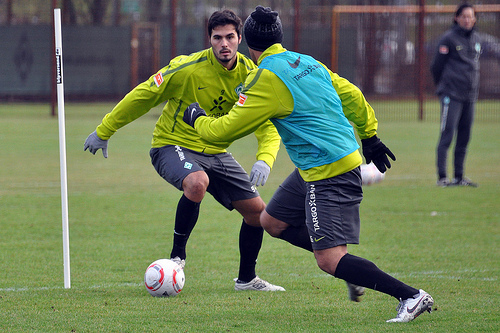
\includegraphics[width=\textwidth]{5369771639}
         \caption{Immagine originale}
     \end{subfigure}
     \begin{subfigure}[b]{0.45\textwidth}
         \centering
         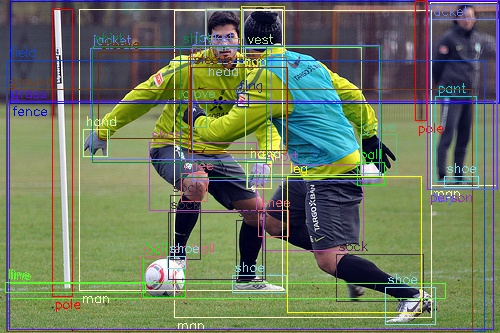
\includegraphics[width=\textwidth]{5369771639_detection.jpg}
         \caption{Object Detection}
     \end{subfigure}
     \begin{subfigure}[b]{0.45\textwidth}
         \centering
         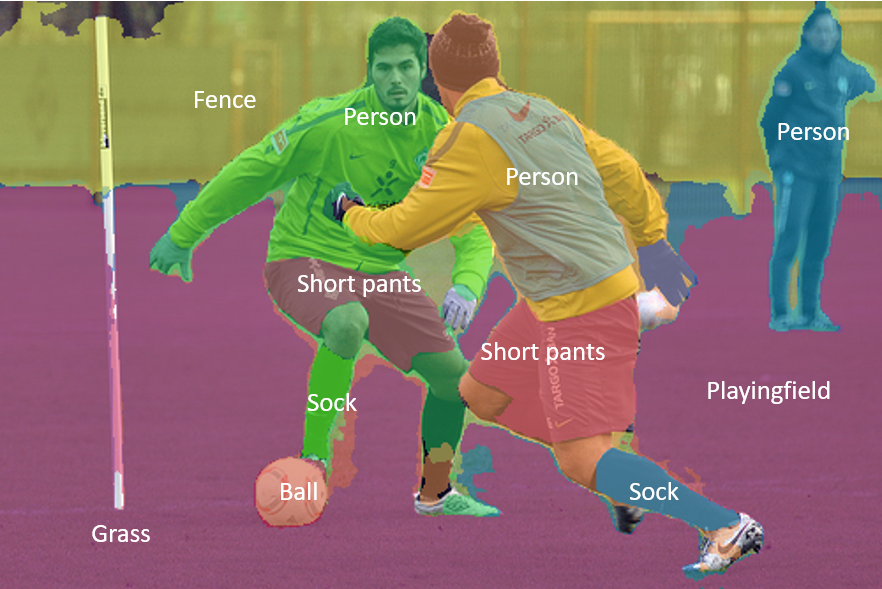
\includegraphics[width=\textwidth]{5369771639_seg}
         \caption{Image Segmentation}
     \end{subfigure}
     \captionsetup{singlelinecheck=off}
        \caption{Illustrazione contenente i risultati delle componenti di image understanding per l'immagine di Flickr30k con id: \textit{5369771639}.
        Caption di riferimento: 1) Two male soccer players in lime green uniforms passing the ball to each other; 2) Two men on opposing teams are playing soccer in a field; 3) Two soccer players going head-to-head for a soccer ball; 4) Two men scrimmage in soccer, as a referee looks on; 5) Two soccer players in long sleeves.\\
        Di seguito vengono riportate le predizioni ottenute in ogni prova effettuata.\\
        \textbf{\acrshort{oscar}$_+$ \acrshort{mtl} seg1*}: \textit{two young men are playing soccer on a field}.\\
        \textbf{\acrshort{oscar}$_+$ \acrshort{scst} seg1*}: \textit{two soccer players, one in green and one in blue, are playing soccer}.\\
        \textbf{\acrshort{oscar}$_+$ \acrshort{mtl} seg2*}: \textit{two men are playing soccer on a field}.\\
        \textbf{\acrshort{oscar}$_+$ \acrshort{scst} seg2*}: \textit{two men are playing soccer on a field}.\\
        \textbf{\acrshort{oscar}$_+$ \acrshort{mtl} seg3*}: \textit{two men playing soccer on a field}.\\
        \textbf{\acrshort{oscar}$_+$ \acrshort{scst} seg3*}: \textit{two men are playing soccer on a field}.\\
        \textbf{\acrshort{oscar}$_+$ \acrshort{mtl} seg+det1*}: \textit{two soccer players in yellow and blue uniforms are playing soccer}.\\
        \textbf{\acrshort{oscar}$_+$ \acrshort{scst} seg+det1*}: \textit{two soccer players in yellow are playing a game}.\\
        \textbf{\acrshort{oscar}$_+$ \acrshort{mtl} seg+det2*}: \textit{two men playing soccer on a field}.\\
        \textbf{\acrshort{oscar}$_+$ \acrshort{scst} seg+det2*}: \textit{two men in yellow shirts are playing soccer on a field}.\\
        \textbf{\acrshort{oscar}$_+$ \acrshort{mtl} seg+det3*}: \textit{two soccer players in yellow and blue uniforms are playing soccer}.\\
        \textbf{\acrshort{oscar}$_+$ \acrshort{scst} seg+det3*}: \textit{two men in yellow and blue uniforms are playing soccer}.\\
        \textbf{\acrshort{oscar}$_+$ \acrshort{mtl} det*}: \textit{two men in yellow and blue uniforms playing soccer}.\\
        \textbf{\acrshort{oscar}$_+$ \acrshort{scst} det*}: \textit{two men in yellow and blue uniforms are playing soccer}.
        }
        \label{fig:test1}
\end{figure}

\begin{figure}[H]
     \centering
     \begin{subfigure}[b]{0.32\textwidth}
         \centering
         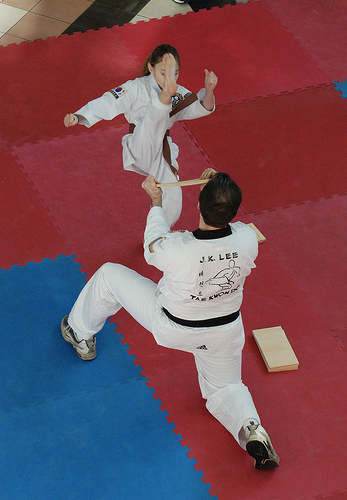
\includegraphics[width=\textwidth]{101362133}
         \caption{Immagine originale}
     \end{subfigure}
     \begin{subfigure}[b]{0.32\textwidth}
         \centering
         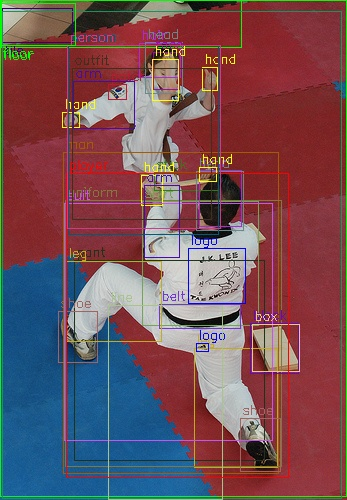
\includegraphics[width=\textwidth]{101362133_detection.jpg}
         \caption{Object Detection}
     \end{subfigure}
     \begin{subfigure}[b]{0.32\textwidth}
         \centering
         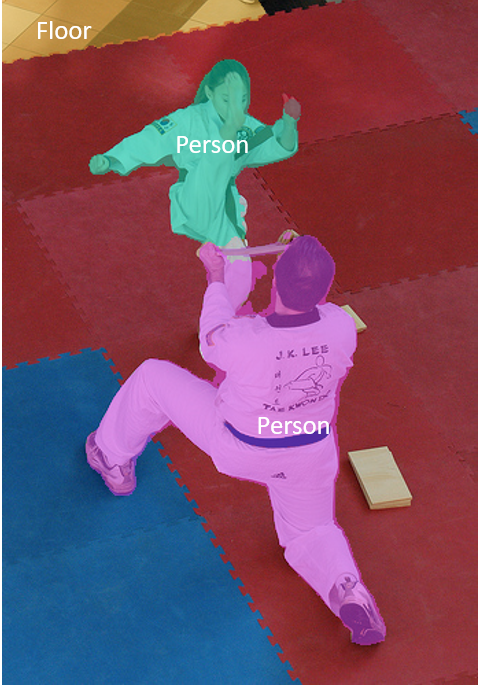
\includegraphics[width=\textwidth]{101362133_seg}
         \caption{Image Segmentation}
     \end{subfigure}
     \captionsetup{singlelinecheck=off}
        \caption{Illustrazione contenente i risultati delle componenti di image understanding per l'immagine di Flickr30k con id: \textit{101362133}.
        Caption di riferimento: 1) A young female student performing a downward kick to break a board held by her Karate instructor; 2) Girl about to kick a piece of wood in half while karate instructor holds it; 3) A girl kicking a stick that a man is holding in tae kwon do class; 4) A girl in karate uniform breaking a stick with a front kick; 5) A girl breaking boards by using karate.\\
        Di seguito vengono riportate le predizioni ottenute in ogni prova effettuata.\\
        \textbf{\acrshort{oscar}$_+$ \acrshort{mtl} seg1*}: \textit{two men are competing in a martial arts match}.\\
        \textbf{\acrshort{oscar}$_+$ \acrshort{scst} seg1*}: \textit{two men are performing a martial arts move on the floor}.\\
        \textbf{\acrshort{oscar}$_+$ \acrshort{mtl} seg2*}: \textit{two men are competing in a martial arts match}.\\
        \textbf{\acrshort{oscar}$_+$ \acrshort{scst} seg2*}: \textit{two men are performing a martial arts move on the floor}.\\
        \textbf{\acrshort{oscar}$_+$ \acrshort{mtl} seg3*}: \textit{two men, one in a white shirt and one in a black shirt, are fighting}.\\
        \textbf{\acrshort{oscar}$_+$ \acrshort{scst} seg3*}: \textit{two young men are practicing martial arts on the floor}.\\
        \textbf{\acrshort{oscar}$_+$ \acrshort{mtl} seg+det1*}: \textit{two people are practicing martial arts on a red mat}.\\
        \textbf{\acrshort{oscar}$_+$ \acrshort{scst} seg+det1*}: \textit{two people are practicing martial arts on a red mat}.\\
        \textbf{\acrshort{oscar}$_+$ \acrshort{mtl} seg+det2*}: \textit{two people are practicing martial arts on a red mat}.\\
        \textbf{\acrshort{oscar}$_+$ \acrshort{scst} seg+det2*}: \textit{two people are practicing martial arts on a red mat}.\\
        \textbf{\acrshort{oscar}$_+$ \acrshort{mtl} seg+det3*}: \textit{two people are practicing martial arts on a red mat}.\\
        \textbf{\acrshort{oscar}$_+$ \acrshort{scst} seg+det3*}: \textit{two people are practicing martial arts on a red mat}.\\
        \textbf{\acrshort{oscar}$_+$ \acrshort{mtl} det*}: \textit{two people are practicing martial arts on a red mat}.\\
        \textbf{\acrshort{oscar}$_+$ \acrshort{scst} det*}: \textit{two people are practicing martial arts on a red mat}.
        }
        \label{fig:test2}
\end{figure}


\begin{figure}[H]
     \centering
     \begin{subfigure}[b]{0.31\textwidth}
         \centering
         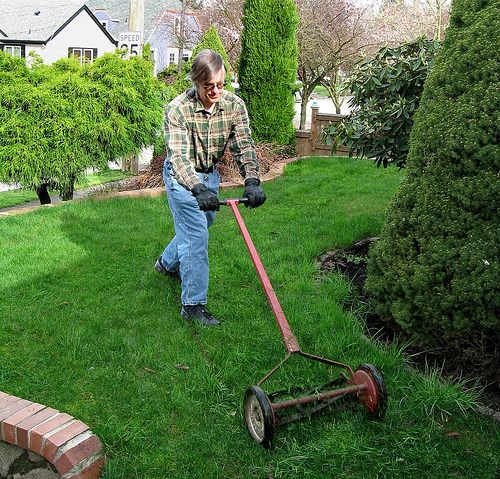
\includegraphics[width=\textwidth]{4434125934}
         \caption{Immagine originale}
     \end{subfigure}
     \begin{subfigure}[b]{0.31\textwidth}
         \centering
         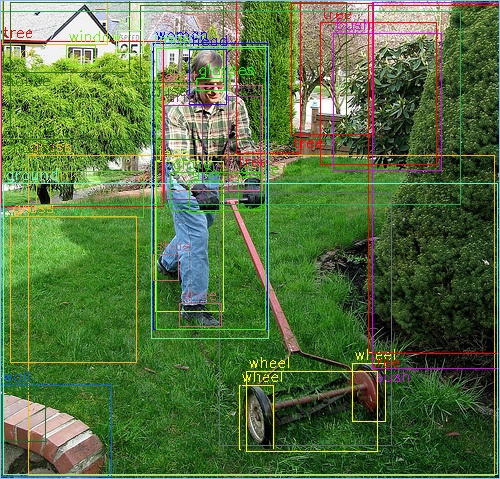
\includegraphics[width=\textwidth]{4434125934_detection.jpg}
         \caption{Object Detection}
     \end{subfigure}
     \begin{subfigure}[b]{0.31\textwidth}
         \centering
         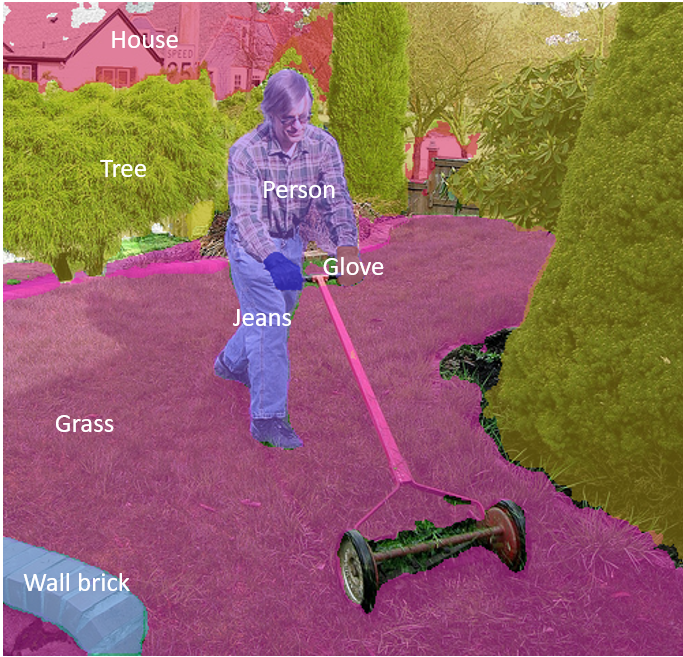
\includegraphics[width=\textwidth]{4434125934_seg}
         \caption{Image Segmentation}
     \end{subfigure}
     \captionsetup{singlelinecheck=off}
        \caption{Illustrazione contenente i risultati delle componenti di image understanding per l'immagine di Flickr30k con id: \textit{4434125934}.
        Caption di riferimento: 1)  A man, dressed in bright blue jeans and a plaid shirt, mows a shaggy green lawn in his cozy suburban front yard; 2) A guy maintains his yard by mowing with a traditional, non-powered lawn mower; 3) A gray-haired man wearing black gloves is moving the lawn; 4) A man mows a small lawn with a push mower; 5) Man in long-sleeve shirt mows his lawn.\\
        Di seguito vengono riportate le predizioni ottenute in ogni prova effettuata.\\
        \textbf{\acrshort{oscar}$_+$ \acrshort{mtl} seg1*}: \textit{a man in a blue shirt is using a chainsaw to cut down a tree}.\\
        \textbf{\acrshort{oscar}$_+$ \acrshort{scst} seg1*}: \textit{a man in a blue shirt is working on a garden}.\\
        \textbf{\acrshort{oscar}$_+$ \acrshort{mtl} seg2*}: \textit{a man in a blue shirt and jeans is digging a hole with a shovel}.\\
        \textbf{\acrshort{oscar}$_+$ \acrshort{scst} seg2*}: \textit{a man in a green shirt is working on a garden}.\\
        \textbf{\acrshort{oscar}$_+$ \acrshort{mtl} seg3*}: \textit{a man in a blue shirt and jeans is digging a hole with a shovel}.\\
        \textbf{\acrshort{oscar}$_+$ \acrshort{scst} seg3*}: \textit{a man in a blue shirt is working on a piece of garden}.\\
        \textbf{\acrshort{oscar}$_+$ \acrshort{mtl} seg+det1*}: \textit{a man in a plaid shirt is mowing the grass with a red mower}.\\
        \textbf{\acrshort{oscar}$_+$ \acrshort{scst} seg+det1*}: \textit{a man in a plaid shirt is mowing the grass with a red mower}.\\
        \textbf{\acrshort{oscar}$_+$ \acrshort{mtl} seg+det2*}: \textit{a woman in a plaid shirt is mowing the grass with a red mower}.\\
        \textbf{\acrshort{oscar}$_+$ \acrshort{scst} seg+det2*}: \textit{a man in a plaid shirt is cutting grass with a red mower}.\\
        \textbf{\acrshort{oscar}$_+$ \acrshort{mtl} seg+det3*}: \textit{a man in a plaid shirt and jeans is mowing a lawn with a red mower}.\\
        \textbf{\acrshort{oscar}$_+$ \acrshort{scst} seg+det3*}: \textit{a man in a plaid shirt and jeans is mowing the lawn with a red mower}.\\
        \textbf{\acrshort{oscar}$_+$ \acrshort{mtl} det*}: \textit{a man in a plaid shirt and blue jeans is mowing the lawn}.\\
        \textbf{\acrshort{oscar}$_+$ \acrshort{scst} det*}: \textit{a man in a plaid shirt is mowing the lawn with a red mower}.
        }
        \label{fig:test3}
\end{figure}

\begin{figure}[H]
     \centering
     \begin{subfigure}[b]{0.45\textwidth}
         \centering
         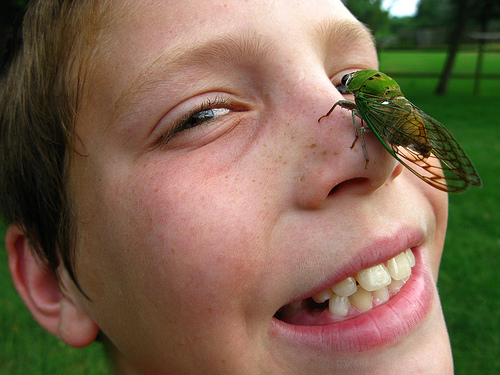
\includegraphics[width=\textwidth]{2750185692}
         \caption{Immagine originale}
     \end{subfigure}
     \begin{subfigure}[b]{0.45\textwidth}
         \centering
         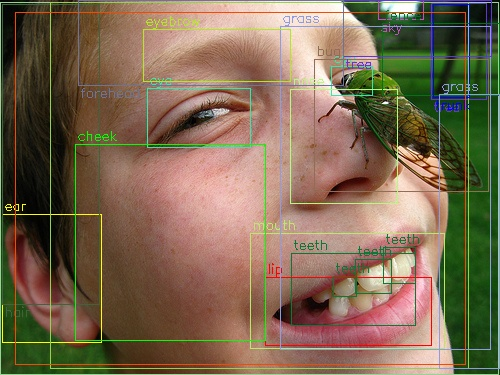
\includegraphics[width=\textwidth]{2750185692_detection.jpg}
         \caption{Object Detection}
     \end{subfigure}
     \begin{subfigure}[b]{0.45\textwidth}
         \centering
         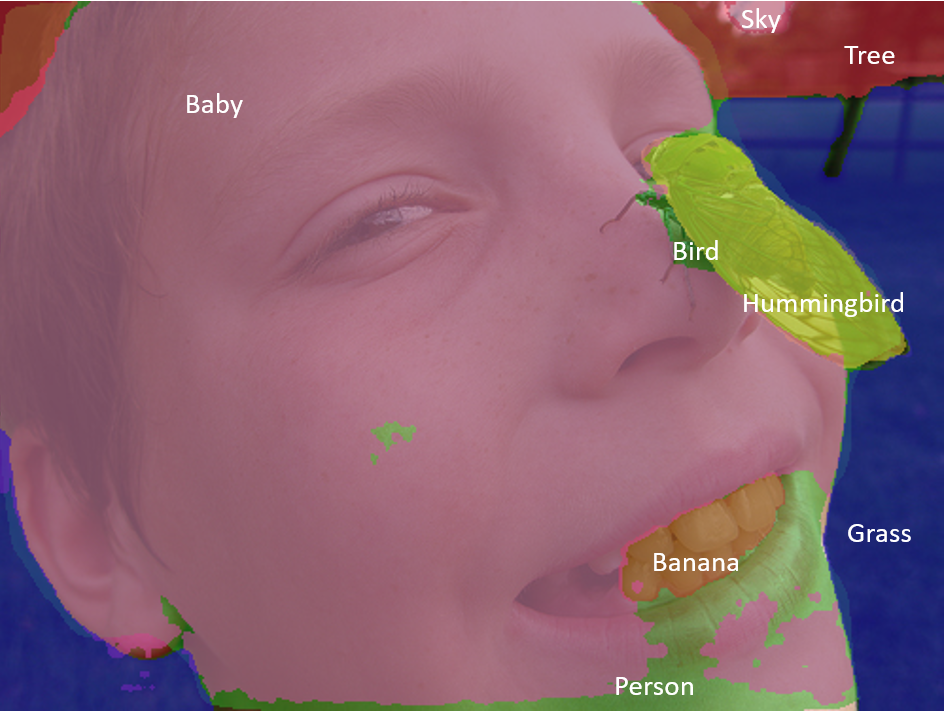
\includegraphics[width=\textwidth]{2750185692_seg}
         \caption{Image Segmentation}
     \end{subfigure}
     \captionsetup{singlelinecheck=off}
        \caption{Illustrazione contenente i risultati delle componenti di image understanding per l'immagine di Flickr30k con id: \textit{2750185692}.
        Caption di riferimento: 1) Young boy smiles as an extremely large kelly green fly perches on his nose; 2) A green beetle is resting upon a freckled nose of a young boy; 3) Boy that is outside with a green bug sitting on his nose; 4) A boy poses with a large green insect on his nose; 5) A boy with a winged bug perched on his nose.\\
        Di seguito vengono riportate le predizioni ottenute in ogni prova effettuata.\\
        \textbf{\acrshort{oscar}$_+$ \acrshort{mtl} seg1*}: \textit{a man in a green shirt is holding a large bird}.\\
        \textbf{\acrshort{oscar}$_+$ \acrshort{scst} seg1*}: \textit{a man is holding a green bird in a tree}.\\
        \textbf{\acrshort{oscar}$_+$ \acrshort{mtl} seg2*}: \textit{a young boy is eating a banana}.\\
        \textbf{\acrshort{oscar}$_+$ \acrshort{scst} seg2*}: \textit{a young boy is holding a bird in his mouth}.\\
        \textbf{\acrshort{oscar}$_+$ \acrshort{mtl} seg3*}: \textit{a young boy is eating a banana}.\\
        \textbf{\acrshort{oscar}$_+$ \acrshort{scst} seg3*}: \textit{a young boy is holding a bird in his hand}.\\
        \textbf{\acrshort{oscar}$_+$ \acrshort{mtl} seg+det1*}: \textit{a young boy is looking at a hummingbird}.\\
        \textbf{\acrshort{oscar}$_+$ \acrshort{scst} seg+det1*}: \textit{a young boy is looking at a hummingbird}.\\
        \textbf{\acrshort{oscar}$_+$ \acrshort{mtl} seg+det2*}: \textit{a young boy is looking at a green insect}.\\
        \textbf{\acrshort{oscar}$_+$ \acrshort{scst} seg+det2*}: \textit{a young boy is looking at a green bug}.\\
        \textbf{\acrshort{oscar}$_+$ \acrshort{mtl} seg+det3*}: \textit{a young boy with a green butterfly on his nose}.\\
        \textbf{\acrshort{oscar}$_+$ \acrshort{scst} seg+det3*}: \textit{a young boy is looking at a green insect on his nose}.\\
        \textbf{\acrshort{oscar}$_+$ \acrshort{mtl} det*}: \textit{a young boy is looking at a green insect}.\\
        \textbf{\acrshort{oscar}$_+$ \acrshort{scst} det*}: \textit{a young boy is looking at a green insect on his nose}.
        }
        \label{fig:test4}
\end{figure}

\begin{figure}[H]
     \centering
     \begin{subfigure}[b]{0.47\textwidth}
         \centering
         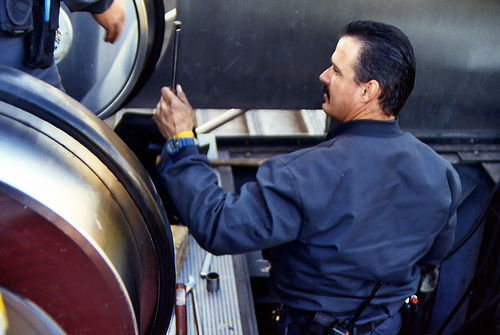
\includegraphics[width=\textwidth]{1989609}
         \caption{Immagine originale}
     \end{subfigure}
     \begin{subfigure}[b]{0.47\textwidth}
         \centering
         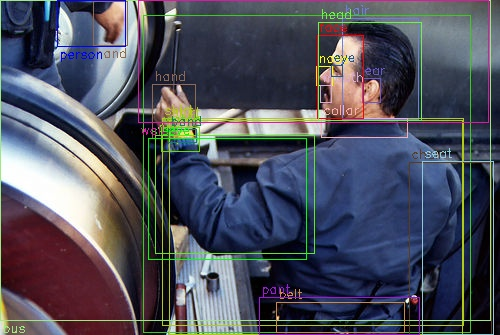
\includegraphics[width=\textwidth]{1989609_detection.jpg}
         \caption{Object Detection}
     \end{subfigure}
     \begin{subfigure}[b]{0.47\textwidth}
         \centering
         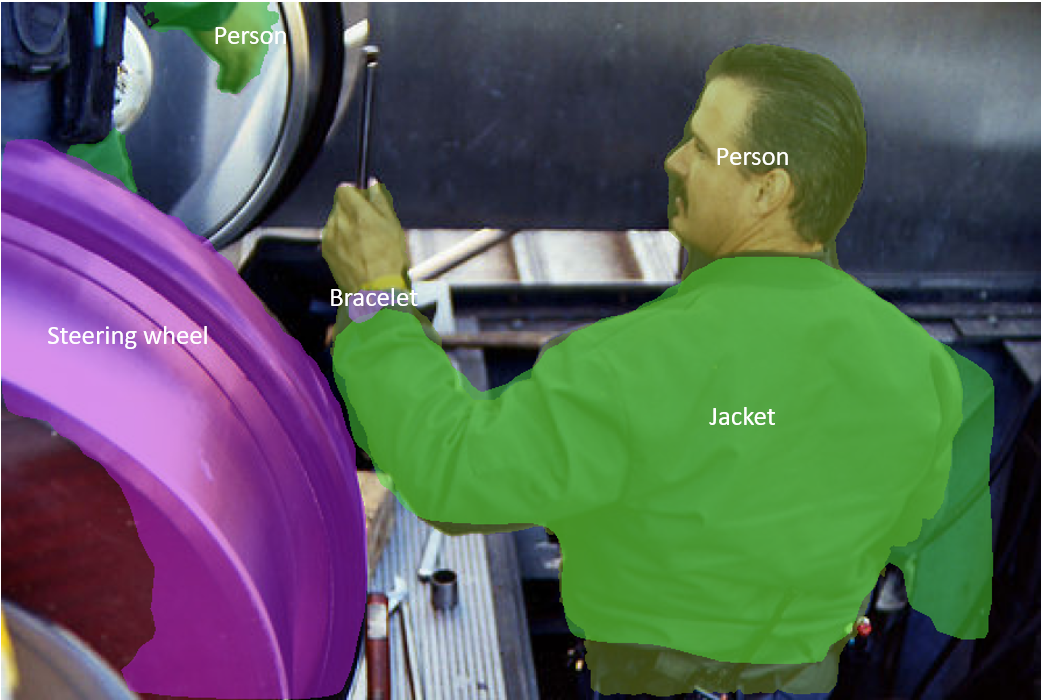
\includegraphics[width=\textwidth]{1989609_seg}
         \caption{Image Segmentation}
     \end{subfigure}
     \captionsetup{singlelinecheck=off}
        \caption{Illustrazione contenente i risultati delle componenti di image understanding per l'immagine di Flickr30k con id: \textit{1989609}.
        Caption di riferimento: 1) A man wearing blue coveralls is handing a tool to another person; 2) A man in a navy blue jacket holding a tool in his dirty hand; 3) A man in a work uniform passing a tool to another person; 4) Man in a blue jumpsuit attempts to repair an escalator; 5) A man with a mustache works on a broken escalator.\\
        Di seguito vengono riportate le predizioni ottenute in ogni prova effettuata.\\
        \textbf{\acrshort{oscar}$_+$ \acrshort{mtl} seg1*}: \textit{a man in a blue jacket is driving a car}.\\
        \textbf{\acrshort{oscar}$_+$ \acrshort{scst} seg1*}: \textit{a man in a blue jacket is driving a car}.\\
        \textbf{\acrshort{oscar}$_+$ \acrshort{mtl} seg2*}: \textit{a man in a blue jacket is driving a car}.\\
        \textbf{\acrshort{oscar}$_+$ \acrshort{scst} seg2*}: \textit{a man in a black jacket is driving a car}.\\
        \textbf{\acrshort{oscar}$_+$ \acrshort{mtl} seg3*}: \textit{a man in a blue jacket is driving a car}.\\
        \textbf{\acrshort{oscar}$_+$ \acrshort{scst} seg3*}: \textit{a man in a blue jacket is driving a car}.\\
        \textbf{\acrshort{oscar}$_+$ \acrshort{mtl} seg+det1*}: \textit{a man in a blue jacket is working on a car}.\\
        \textbf{\acrshort{oscar}$_+$ \acrshort{scst} seg+det1*}: \textit{a man in a blue jacket is standing at the wheel of a car}.\\
        \textbf{\acrshort{oscar}$_+$ \acrshort{mtl} seg+det2*}: \textit{a man in a blue jacket is working on a car}.\\
        \textbf{\acrshort{oscar}$_+$ \acrshort{scst} seg+det2*}: \textit{a man in a blue jacket is working on a car}.\\
        \textbf{\acrshort{oscar}$_+$ \acrshort{mtl} seg+det3*}: \textit{a man in a blue jacket is working on a car}.\\
        \textbf{\acrshort{oscar}$_+$ \acrshort{scst} seg+det3*}: \textit{a man in a blue jacket is working on a car}.\\
        \textbf{\acrshort{oscar}$_+$ \acrshort{mtl} det*}: \textit{a man in a blue shirt is working on a car}.\\
        \textbf{\acrshort{oscar}$_+$ \acrshort{scst} det*}: \textit{a man in a blue shirt is working on a car}.
        }
        \label{fig:test5}
\end{figure}

\begin{figure}[H]
     \centering
     \begin{subfigure}[b]{0.32\textwidth}
         \centering
         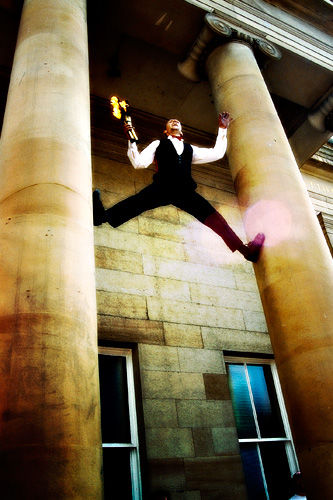
\includegraphics[width=\textwidth]{21138719}
         \caption{Immagine originale}
     \end{subfigure}
     \begin{subfigure}[b]{0.32\textwidth}
         \centering
         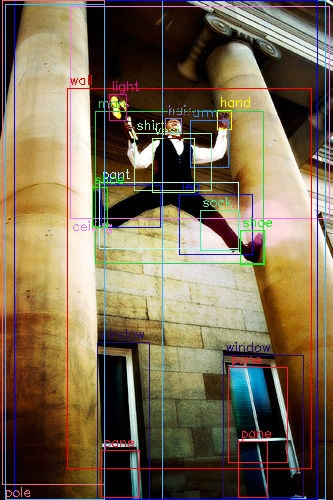
\includegraphics[width=\textwidth]{21138719_detection.jpg}
         \caption{Object Detection}
     \end{subfigure}
     \begin{subfigure}[b]{0.32\textwidth}
         \centering
         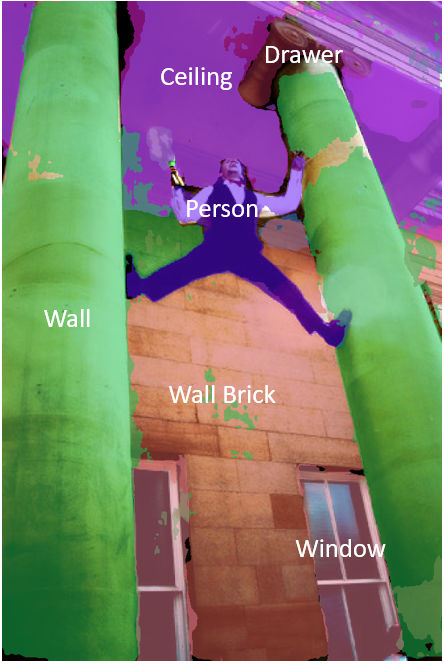
\includegraphics[width=\textwidth]{21138719_seg}
         \caption{Image Segmentation}
     \end{subfigure}
     \captionsetup{singlelinecheck=off}
        \caption{Illustrazione contenente i risultati delle componenti di image understanding per l'immagine di Flickr30k con id: \textit{21138719}.
        Caption di riferimento: 1) Man in black pants and vest balances between to pillars, holding two flaming torches in his right hand; 2) A well-dressed man climbing between two columns while holding torches; 3) A man in a suit is straddling two pillars while holding a flame; 4) Juggler standing balanced between two columns; 5) Man scaling wall with fire in hand.\\
        Di seguito vengono riportate le predizioni ottenute in ogni prova effettuata.\\
        \textbf{\acrshort{oscar}$_+$ \acrshort{mtl} seg1*}: \textit{a man in a black shirt is jumping in the air}.\\
        \textbf{\acrshort{oscar}$_+$ \acrshort{scst} seg1*}: \textit{a man in a black shirt is jumping in the air in a room}.\\
        \textbf{\acrshort{oscar}$_+$ \acrshort{mtl} seg2*}: \textit{a man in a black shirt is jumping in the air on a trampoline}.\\
        \textbf{\acrshort{oscar}$_+$ \acrshort{scst} seg2*}: \textit{a man in a black shirt is jumping on a ladder}.\\
        \textbf{\acrshort{oscar}$_+$ \acrshort{mtl} seg3*}: \textit{a man in a black shirt is jumping in the air on a trampoline}.\\
        \textbf{\acrshort{oscar}$_+$ \acrshort{scst} seg3*}: \textit{a man in a white shirt is jumping in the air on a ladder}.\\
        \textbf{\acrshort{oscar}$_+$ \acrshort{mtl} seg+det1*}: \textit{a man is hanging upside down from a rope}.\\
        \textbf{\acrshort{oscar}$_+$ \acrshort{scst} seg+det1*}: \textit{a man in a black shirt is hanging from a pipe}.\\
        \textbf{\acrshort{oscar}$_+$ \acrshort{mtl} seg+det2*}: \textit{a man is hanging upside down from a rope}.\\
        \textbf{\acrshort{oscar}$_+$ \acrshort{scst} seg+det2*}: \textit{a man is hanging upside down from a building}.\\
        \textbf{\acrshort{oscar}$_+$ \acrshort{mtl} seg+det3*}: \textit{a man is jumping in the air between two columns}.\\
        \textbf{\acrshort{oscar}$_+$ \acrshort{scst} seg+det3*}: \textit{a man in a black suit is jumping between two columns}.\\
        \textbf{\acrshort{oscar}$_+$ \acrshort{mtl} det*}: \textit{a man is jumping in the air between two columns}.\\
        \textbf{\acrshort{oscar}$_+$ \acrshort{scst} det*}: \textit{a man in a black suit is jumping between two columns}.
        }
        \label{fig:test6}
\end{figure}
\newpage

\section{Considerazioni}\label{considerazioni}
I modelli ottenuti tramite la componente di Image Segmentation hanno ottenuto le performance più basse, però come si è visto nella Sezione \ref{analisi_qualitativa} sono stati in grado di produrre didascalie di discreta qualità dove è comunque comprensibile il contenuto visivo dell'immagine. Inoltre, come si è potuto vedere dai risultati il fine-tuning tramite \acrshort{scst} è molto utile, poichè permette di ottenere delle didascalie di qualità superiore. 


Analizzando l'andamento della loss function dei modelli che usano l'ensemble di Image Segmentation è stata osservata una discesa più accentuata rispetto alla versione che usa i modelli di Object Detection. Infatti, è stata effettuata una prova in cui sono stati allenati i modelli con alcune epoche aggiuntive e sono stati notati dei miglioramenti più marcati nella versione che usa la segmentazione. Quest'ultima osservazione non è stata applicata su tutti i modelli per effettuare delle comparazioni eque, che considerano gli stessi parametri per tutte le prove, e perché il fine-tuning dei modelli richiede molto tempo (basti pensare che ogni fine-tuning effettuato ha richiesto più di sei giorni per il completamento).


Le prove che prevedono la componente di Image Segmentation (da sola o in combinazione, ad eccezione della prova seg+det3) hanno ottenuto dei risultati bassi sulla metrica \acrshort{bleu}@4. La principale motivazione deriva dal fatto che questa metrica si basa sulla precisione dei termini utilizzati, molto spesso le classi individuate tramite segmentazione sono poco accurate e le caption prodotte contengono termini più generici e sinonimi.
Inoltre, la combinazione tra tutte le feature estratte tramite Image Segmentation con tutte quelle estratte tramite Object Detection ha ottenute le performance più elevate su tre metriche ad eccezione della \acrshort{cider}. Analizzando le didascalie prodotte non è stata trovata una grossa differenza ad eccezione di qualche dettaglio (per esempio la Figura \ref{fig:test5}), poichè la differenza è minima è stato difficile trovare la possibile causa.

Infine, una cosa molto importate da considerare è che spesso le caption generate non sono molto fedeli a quelle di riferimento, questo è dovuto principalmente al fatto che le didascalie di riferimento contengono informazioni implicite, contestuali e altri aspetti difficili da catturare considerando solo gli oggetti presenti nell'immagine.